% Packages
\usepackage{mdframed}
\usepackage{multirow} %% Pour mettre un texte sur plusieurs rangées
\usepackage{multicol} %% Pour mettre un texte sur plusieurs colonnes
\usepackage{scrextend} %Forcer la 4ème  de couverture en page pair
\usepackage{tikz}
\usepackage{graphicx}
\usepackage[absolute]{textpos}
\usepackage{colortbl}
\usepackage{array}
\usepackage{geometry}
\usepackage{titlesec}
\usepackage[backref=page]{hyperref}
\hypersetup{ % paramétrage couleur des liens hypertextes, toujours garder colorlinks=true
    colorlinks=true,
    linkcolor=black,
    urlcolor=purple}
\usepackage[full]{textcomp}
\usepackage{gensymb}
\usepackage[utf8]{inputenc}
\usepackage[T1]{fontenc}
\usepackage[french,main=english]{babel}
\usepackage[default, scale=.95]{opensans} % police Open Sans
\usepackage{amsmath}
\usepackage{amsfonts}
\usepackage{fancyhdr}
\usepackage{amssymb}
\usepackage{xcolor} % où color selon l'installation
\usepackage[inline]{enumitem}
\usepackage{csquotes}
\usepackage{overpic}
\usepackage{lipsum}
\usepackage{xspace}
\usepackage{xpunctuate}
\usepackage{subcaption}
\usepackage{tabularx}
\usepackage{flushend}
\usepackage[export]{adjustbox}
\usepackage{graphbox}
\usepackage{cite}
\usepackage{comment}
\usepackage{varwidth} %for the varwidth minipage environment
\usepackage{wrapfig}
\usepackage{stix2}
\usepackage{pifont}% http://ctan.org/pkg/pifont
\usepackage{minitoc} %For table of content at each chapter
%\usepackage{natbib}
%\usepackage{bibentry}

%\usepackage[backend=bibtex,style=numeric]{biblatex}
%\usepackage[backend=biber,style=numeric]{biblatex}
%\addbibresource{bibliography.bib}

% Colors
\definecolor{Prune}{RGB}{99,0,60} % l14-33 : couleurs de la charte graphique upsaclay
\definecolor{B1}{RGB}{49,62,72}
\definecolor{C1}{RGB}{124,135,143}
\definecolor{D1}{RGB}{213,218,223}
\definecolor{A2}{RGB}{198,11,70}
\definecolor{B2}{RGB}{237,20,91}
\definecolor{C2}{RGB}{238,52,35}
\definecolor{D2}{RGB}{243,115,32}
\definecolor{A3}{RGB}{124,42,144}
\definecolor{B3}{RGB}{125,106,175}
\definecolor{C3}{RGB}{198,103,29}
\definecolor{D3}{RGB}{254,188,24}
\definecolor{A4}{RGB}{0,78,125}
\definecolor{B4}{RGB}{14,135,201}
\definecolor{C4}{RGB}{0,148,181}
\definecolor{D4}{RGB}{70,195,210}
\definecolor{A5}{RGB}{0,128,122}
\definecolor{B5}{RGB}{64,183,105}
\definecolor{C5}{RGB}{140,198,62}
\definecolor{D5}{RGB}{213,223,61}
\definecolor{lightgrey}{gray}{0.9}

% For network schemas
\colorlet{temoin}{teal!80!white!50}
\colorlet{parent}{yellow!80!white!50}
\colorlet{epoux}{orange!80!white!50}
\colorlet{epouse}{purple!80!white!50}

% Collaboration IDS
\newcommand{\pascal}{\#1\xspace}
\newcommand{\nicole}{\#2\xspace}
\newcommand{\zacarias}{\#3\xspace}
\newcommand{\dana}{\#4\xspace}
\newcommand{\myindent}{~~} % ~\rule{1pt}{6pt}


\newcommand{\cmark}{\ding{51}}%
\newcommand{\xmark}{\ding{55}}%
\newcommand{\rev}[1]{#1}
\newenvironment{revs}{}{}
\newcommand{\del}[1]{}
\newcommand{\ie}{i.e.\xcomma}
\newcommand{\eg}{e.g.\xcomma}
\newcommand{\paovis}{PAOHVis\xspace}

\def\Snospace~{\S{}} % eat the ~ added by \autoref after the macro
\renewcommand*\sectionautorefname{\Snospace}
\renewcommand*\subsectionautorefname{\Snospace}
\renewcommand*\subsubsectionautorefname{\Snospace}

\newcommand{\alexis}[1]{\textcolor{red}{alexis: #1}}
\newcommand{\jdf}[1]{\textcolor{blue}{jdf: #1}}
\newcommand{\christophe}[1]{\textcolor{green}{christophe: #1}}

\newcommand*\circled[1]{\tikz[baseline=(char.base)]{
            \node[shape=circle,draw,inner sep=2pt] (char) {#1};}}
\newcommand*\circledColored[2]{\tikz[baseline=(char.base)]{
            \node[#2,shape=circle,draw,inner sep=2pt] (char) {#1};}}
\newcommand{\ts}{\textsuperscript}

\newcommand{\model}{bipartite multivariate dynamic network\xspace}
\newcommand{\modelplural}{bipartite multivariate dynamic networks\xspace}

\newcommand{\todo}[1]{\textcolor{red}{\textbf{#1}}}
\newcommand{\name}{ComBiNet\xspace}

% Terms
\newcommand{\hsna}{HSNA\xspace}
\newcommand{\sna}{SNA\xspace}
\newcommand{\va}{VA\xspace}
\newcommand{\eda}{Exploratory Data Analysis\xspace}
\newcommand{\snv}{social network visualization\xspace}

% Research Questions
\newcommand{\qone}{\textbf{Q1}\xspace}
\newcommand{\qtwo}{\textbf{Q2}\xspace}
\newcommand{\qthree}{\textbf{Q3}\xspace}

\newcommand{\paperbox}[1]{
\vspace{1em}
\noindent\fbox{\begin{minipage}{\textwidth}
#1
\end{minipage}}
% \vspace{1pt}
}

% Square scales commands
\newcommand{\scalezero}{$\smwhtsquare \smwhtsquare \smwhtsquare$}
\newcommand{\scaleone}{$\smblksquare \smwhtsquare \smwhtsquare$}
\newcommand{\scaletwo}{$\smblksquare \smblksquare \smwhtsquare$}
\newcommand{\scalethree}{$\smblksquare \smblksquare \smblksquare$}


% GRAPHLETS
\newcommand{\inlinevisImproved}[3]{\raisebox{#1}[0pt][0pt]{\includegraphics[height=#2]{#3}}}

\newcommand{\EDGE}{\inlinevisImproved{-3pt}{1.1em}{static/figures/RelatedWork/graphlets/edge.pdf}}
\newcommand{\PATH}{\inlinevisImproved{-3pt}{1.1em}{static/figures/RelatedWork/graphlets/edge2.pdf}}
\newcommand{\TRIANGLE}{\inlinevisImproved{-3pt}{1.1em}{static/figures/RelatedWork/graphlets/triangle.pdf}}




% FOR HSNA PROCESS CHAPTER
\newcommand{\simple}[1][0]{\begin{tikzpicture}[node distance=3cm, auto, every node/.style={inner sep=3,outer sep=0}]
        \node[shape=circle,draw=gray, fill=lightgrey] (A) at (0,1) {\tiny H};
        \node[shape=circle,draw=gray, fill=lightgrey] (B) at (2,1) {\tiny W};
        \node[shape=circle,draw=gray, fill=lightgrey] (T1) at (1,2) {\tiny T1};
        \node[shape=circle,draw=gray, fill=lightgrey] (T2) at (1,0) {\tiny T2};

        \begin{scope}[every node/.style={scale=.5}]
            \path [line width=0.5mm]
            (A)  edge node [color=black] {\small 1659} (B)
            (T1) edge node [color=black] {\small 1659} (T2)
            (T1) edge node [above left, color=black] {\small 1659} (A)
            (T1) edge node [color=black] {\small 1659} (B)
            (T2) edge node [color=black] {\small 1659} (A)
            (T2) edge node [right, color=black] {\small 1659} (B);
        \end{scope}
    \end{tikzpicture}}


\newcommand{\noParents}[1][0]{\begin{tikzpicture}[->, node distance=3cm, auto, every node/.style={inner sep=3,outer sep=0}]
        \node[shape=circle,draw=gray, fill=lightgrey] (A) at (0,1) {\tiny H};
        \node[shape=circle,draw=gray, fill=lightgrey] (B) at (2,1) {\tiny W};
        \node[shape=circle,draw=gray, fill=lightgrey] (T1) at (1,2) {\tiny T1};
        \node[shape=circle,draw=gray, fill=lightgrey] (T2) at (1,0) {\tiny T2};

        \begin{scope}[every node/.style={scale=.5}]
            \path [line width=0.5mm] (A) edge [bend left, color=epoux] node [color=black] {\small 1712} (B)
            (B) edge [bend left, color=epouse] node [color=black] {\small 1659} (A)
            (T1) edge [color=temoin] node [above left, color=black] {\small 1659} (A)
            (T1) edge [color=temoin] node [color=black] {\small 1659} (B)
            (T2) edge [color=temoin] node [color=black] {\small 1659} (A)
            (T2) edge [color=temoin] node [right, color=black] {\small 1659} (B);
        \end{scope}
    \end{tikzpicture}}

% \newcommand{\bipartiteNoParents}[1]{\begin{tikzpicture}[, node distance=3cm, auto, scale=#1]
\newcommand{\bipartiteNoParents}[1][0]{\begin{tikzpicture}[, node distance=3cm, auto, every node/.style={inner sep=3,outer sep=0}]
        \node[shape=circle,draw=gray, fill=lightgrey] (A) at (0,3) {\tiny H};
        \node[shape=circle,draw=gray, fill=lightgrey] (B) at (0,1) {\tiny W};

        \node[shape=circle,draw=gray, fill=lightgrey] (T1) at (2,3) {\tiny T1};
        \node[shape=circle,draw=gray, fill=lightgrey] (T2) at (2,1) {\tiny T2};

        \node[shape=rectangle,draw=gray, align=center,fill=lightgrey] (D) at (1,2) {\tiny M \\[0.5em] \tiny 1659};
        \draw (D.west) -- (D.east);

        \begin{scope}[every node/.style={scale=.5}]
            \path [line width=0.5mm] (A) edge [color=epoux] (D)
            (B) edge [color=epouse] (D)
            (T1) edge [color=temoin] (D)
            (T2) edge [color=temoin] (D);
        \end{scope}
        \end{tikzpicture}}

\newcommand{\unipartiteParents}[1][0]{
\begin{tikzpicture}[->, node distance=3cm, auto]
        \node[shape=circle,draw=gray, fill=lightgrey] (A) at (2,1) {\tiny A};
        \node[shape=circle,draw=gray, fill=lightgrey] (B) at (4,1) {\tiny B};

        \node[shape=circle,draw=gray, fill=lightgrey] (T1) at (3,2) {\tiny T1};
        \node[shape=circle,draw=gray, fill=lightgrey] (T2) at (3,0) {\tiny T2};

        \node[shape=circle,draw=gray, fill=lightgrey] (PA) at (1,2) {\tiny PA};
        \node[shape=circle,draw=gray, fill=lightgrey] (MA) at (1,0) {\tiny MA};

        \node[shape=circle,draw=gray, fill=lightgrey] (PB) at (5,2) {\tiny PB};
        \node[shape=circle,draw=gray, fill=lightgrey] (MB) at (5,0) {\tiny MB};

    \begin{scope}[every node/.style={scale=.5}]
        \path [line width=0.5mm] (A) edge [bend left, color=epoux] node [color=black] {\small 1712} (B)
        (B) edge [bend left, color=epouse] node [color=black] {\small 1712} (A)
        (T1) edge [color=temoin] node [above left, color=black] {\small 1712} (A)
        (T1) edge [color=temoin] node [color=black] {\small 1712} (B)
        (T2) edge [color=temoin] node [color=black] {\small 1712} (A)
        (T2) edge [color=temoin] node [right, color=black] {\small 1712} (B)
        (PA) edge [color=parent] node [color=black] {\small Valencia} (A)
        (MA) edge [color=parent] node [right, color=black] {\small Valencia} (A)
        (PB) edge [color=parent] node [color=black] {\small Valencia} (B)
        (MB) edge [color=parent] node [right, color=black] {\small Valencia} (B);
    \end{scope}
    \end{tikzpicture}
}

\newcommand{\bipartiteParents}[1]{
\begin{tikzpicture}[, node distance=3cm, auto, scale=#1]
        \node[shape=circle,draw=gray, fill=lightgrey] (A) at (0,3) {\tiny H};
        \node[shape=circle,draw=gray, fill=lightgrey] (T1) at (0,2) {\tiny T1};

        \node[shape=circle,draw=gray, fill=lightgrey] (T2) at (0,1) {\tiny T2};
        \node[shape=circle,draw=gray, fill=lightgrey] (B) at (0,0) {\tiny W};

        \node[shape=rectangle,draw=gray, align=center, fill=lightgrey] (D) at (1.5,1.5) {\tiny M \\[0.5em] \tiny 1761};

        \node[shape=rectangle,draw=gray, align=center, fill=lightgrey] (BA) at (1.5,3) {\tiny BA};
        \node[shape=rectangle,draw=gray, align=center, fill=lightgrey] (BB) at (1.5,0) {\tiny BB};
%        \node[shape=rectangle,draw=gray, align=center, fill=lightgrey] (BA) at (1.5,3) {\tiny BA \\[0.5em] \tiny Valencia};
%        \node[shape=rectangle,draw=gray, align=center, fill=lightgrey] (BB) at (1.5,0) {\tiny BB \\[0.5em] \tiny Valencia};

        \draw (D.west) -- (D.east);
        \draw (BA.west) -- (BA.east);
        \draw (BB.west) -- (BB.east);

        \node[shape=circle,draw=gray, fill=lightgrey] (PA) at (3,3) {\tiny HF};
        \node[shape=circle,draw=gray, fill=lightgrey] (MA) at (3,2) {\tiny HM};
        \node[shape=circle,draw=gray, fill=lightgrey] (PB) at (3,1) {\tiny WF};
        \node[shape=circle,draw=gray, fill=lightgrey] (MB) at (3,0) {\tiny WM};

    \begin{scope}[every node/.style={scale=.5}]
        \path [line width=0.5mm] (A) edge [color=epoux] (D)
        (B) edge [color=epouse] (D)
        (T1) edge [color=temoin] (D)
        (T2) edge [color=temoin] (D)
        (PA) edge [color=parent] (BA)
        (MA) edge [color=parent] (BA)
        (PB) edge [color=parent] (BB)
        (MB) edge [color=parent] (BB)
        (A) edge [color=parent] (BA)
        (B) edge [color=parent] (BB);
    \end{scope}
    \end{tikzpicture}
}


\newcommand{\bipartiteParentsOneEvent}[1]{
\begin{tikzpicture}[, node distance=3cm, auto, scale=#1]
        \node[shape=circle,draw=gray, fill=lightgrey] (A) at (0,3) {\tiny H};
        \node[shape=circle,draw=gray, fill=lightgrey] (T1) at (0,2) {\tiny T1};

        \node[shape=circle,draw=gray, fill=lightgrey] (T2) at (0,1) {\tiny T2};
        \node[shape=circle,draw=gray, fill=lightgrey] (B) at (0,0) {\tiny W};

        \node[shape=rectangle,draw=gray, align=center, fill=lightgrey] (D) at (1.5,1.5) {\tiny M \\[0.5em] \tiny 1761};

        \draw (D.west) -- (D.east);

        \node[shape=circle,draw=gray, fill=lightgrey] (PA) at (3,3) {\tiny HF};
        \node[shape=circle,draw=gray, fill=lightgrey] (MA) at (3,2) {\tiny HM};
        \node[shape=circle,draw=gray, fill=lightgrey] (PB) at (3,1) {\tiny WF};
        \node[shape=circle,draw=gray, fill=lightgrey] (MB) at (3,0) {\tiny WM};

    \begin{scope}[every node/.style={scale=.5}]
        \path [line width=0.5mm] (A) edge [color=epoux] (D)
        (B) edge [color=epouse] (D)
        (T1) edge [color=temoin] (D)
        (T2) edge [color=temoin] (D)
        (PA) edge [color=parent] (D)
        (MA) edge [color=parent] (D)
        (PB) edge [color=parent] (D)
        (MB) edge [color=parent] (D);
    \end{scope}
    \end{tikzpicture}
}



\iffalse
\begin{figure}
    \centering

%     \begin{subfigure}{0.5\columnwidth}
%     \includegraphics[width=\columnwidth]{Figures/marriageDocumentnoParents.pdf}
%     % \caption{First, an exciting contribution by unknown artist.}
%   \end{subfigure}
%   \begin{subfigure}{0.32\columnwidth}
%     \bipartiteNoParents{1}
% %   \includegraphics[width=\linewidth]{Figures/marriageDocumentnoParents.pdf}
% %   \resizebox{0.5\textwidth}{!}{
% %     \bipartiteNoParents{1}
% % }%
%     % \caption{Second, an anonymous mystery.}
%   \end{subfigure}
%   \begin{subfigure}{0.5\columnwidth}
%     \includegraphics[width=\linewidth]{Figures/marriageDocument.pdf}
%   \end{subfigure}
%   \begin{subfigure}{0.3\columnwidth}
%     \bipartiteParents{1}
%   \end{subfigure}


  \begin{subfigure}{.23\textwidth}
    \includegraphics[width=\linewidth]{static/figures/HSNAProcess/OriginalPaperFigures/marriageDocumentnoParents.pdf}
    \caption{}
  \end{subfigure}
  \begin{subfigure}{.23\textwidth}
    \centering
    \bipartiteNoParents{1}
  \end{subfigure}
  \begin{subfigure}{.23\textwidth}
        \includegraphics[width=\linewidth]{static/figures/HSNAProcess/OriginalPaperFigures/marriageDocument.pdf}
    \caption{}
%    \includegraphics[scale=0.2,left]{Figures/MarriageLegend.pdf}
        \includegraphics[width=\linewidth]{static/figures/HSNAProcess/OriginalPaperFigures/MarriageLegend.pdf}
  \end{subfigure}
  \centering
  \begin{subfigure}{.23\textwidth}
    \bipartiteParents{1}
  \end{subfigure}


    % \includegraphics[width=0.49\linewidth]{Figures/marriageDocumentnoParents.pdf}
    % \bipartiteNoParents{1}
    % % \subfigure[]{\bipartiteNoParents{0.6}}

    % \includegraphics[width=0.49\linewidth]{Figures/marriageDocument.pdf}
    % \bipartiteParents{1}

    \caption{Transformation of annotated marriage acts from use case \zacarias\ into our proposed model. The acts can refers to parent relationships (b) or not (a). Each color represent a relationship between a person and an event. Additional information on the persons or the events are underlined and stored in the nodes as attributes. The network is a concrete representation of the events mentioned in the original sources. H: Husband, W: wife, T1,T2: witnesses, M: marriage act, HF, HM, WF, WM: husband/wife's father/mother.
    % \jdf{Tu peux expliquer les A, B, T1, T2, PA, MA, PB, MB?}
    }\label{tab:MarriageModel}
\end{figure}
\fi


\colorlet{associate}{orange!80!white!50}
\colorlet{guarantor}{blue!80!white!50}
\colorlet{approbator}{olive!80!white!50}


%\newcommand{\simplePiemont}[1][0]{\begin{tikzpicture}[auto]
\newcommand{\simplePiemont}[1][0]{\begin{tikzpicture}[auto, every node/.style={inner sep=3,outer sep=0}]
        \node[shape=circle,draw=gray, fill=lightgrey] (A1) at (2,1) {\tiny A1};
        \node[shape=circle,draw=gray, fill=lightgrey] (A2) at (2.5,3) {\tiny A2};
        \node[shape=circle,draw=gray, fill=lightgrey] (A3) at (3,1) {\tiny A3};
        \node[shape=circle,draw=gray, fill=lightgrey] (G) at (1.5,2.1) {\tiny G};
%        \node[shape=circle,draw=gray, fill=lightgrey] (G) at (0,2.1) {\tiny G};
        \node[shape=circle,draw=gray, fill=lightgrey] (Ap) at (3.5,2.1) {\tiny Ap};

        \begin{scope}[every node/.style={scale=.5}]
            \path [line width=0.5mm]
            (A1) edge node [above left, color=black] {\small 1712} (A2)
            (A1) edge node [color=black] {\small 1712} (A3)
            (A2) edge node [color=black] {\small 1712} (A3)
            (G) edge node [right, color=black] {\small 1712} (A1)
            (G) edge node [right, color=black] {\small 1712} (A2)
            (G) edge node [right, color=black] {\small 1712} (A3)
            (Ap) edge node [right, color=black] {\small 1712} (A1)
            (Ap) edge node [right, color=black] {\small 1712} (A2)
            (Ap) edge node [right, color=black] {\small 1712} (A3)
            (G) edge node [color=black] {\small 1712} (Ap);
        \end{scope}
    \end{tikzpicture}}

\newcommand{\unipartitePiemont}[1][0]{\begin{tikzpicture}[->, node distance=3cm, auto, every node/.style={inner sep=3,outer sep=0}]
        \node[shape=circle,draw=gray, fill=lightgrey] (A1) at (2,1) {\tiny A1};
        \node[shape=circle,draw=gray, fill=lightgrey] (A2) at (2.5,3) {\tiny A2};
        \node[shape=circle,draw=gray, fill=lightgrey] (A3) at (3,1) {\tiny A3};
        \node[shape=circle,draw=gray, fill=lightgrey] (G) at (1.5,2.1) {\tiny G};
        \node[shape=circle,draw=gray, fill=lightgrey] (Ap) at (3.5,2.1) {\tiny Ap};

        \begin{scope}[every node/.style={scale=.5}]
            \path [line width=0.5mm]
            (A1) edge [color=associate] node [above left, color=black] {\small 1712} (A2)
            (A1) edge [color=associate] node [color=black] {\small 1712} (A3)
            (A2) edge [color=associate] node [color=black] {\small 1712} (A3)
            (G) edge [color=guarantor] node [right, color=black] {\small 1712} (A1)
            (G) edge [color=guarantor] node [right, color=black] {\small 1712} (A2)
            (G) edge [color=guarantor] node [right, color=black] {\small 1712} (A3)
            (Ap) edge [color=approbator] node [right, color=black] {\small 1712} (A1)
            (Ap) edge [color=approbator] node [right, color=black] {\small 1712} (A2)
            (Ap) edge [color=approbator] node [right, color=black] {\small 1712} (A3);
        \end{scope}
    \end{tikzpicture}}


\newcommand{\bipartitePiemont}[1][0]{\begin{tikzpicture}[, node distance=3cm, auto, every node/.style={inner sep=3,outer sep=0}]
        \node[shape=circle,draw=gray, fill=lightgrey] (A1) at (0,3) {\tiny A1};
        \node[shape=circle,draw=gray, fill=lightgrey] (A2) at (0,2) {\tiny A2};
        \node[shape=circle,draw=gray, fill=lightgrey] (A3) at (0,1) {\tiny A3};

        \node[shape=circle,draw=gray, fill=lightgrey] (G) at (2,3) {\tiny G};
        \node[shape=circle,draw=gray, fill=lightgrey] (Ap) at (2,1) {\tiny Ap};

        \node[shape=rectangle,draw=gray, align=center,fill=lightgrey] (D) at (1,2) {\tiny M \\[0.5em] \tiny 1761};
        \draw (D.west) -- (D.east);

        \begin{scope}[every node/.style={scale=.5}]
            \path [line width=0.5mm] (A1) edge [color=associate] (D)
            (A2) edge [color=associate] (D)
            (A3) edge [color=associate] (D)
            (G) edge [color=guarantor] (D)
            (Ap) edge [color=approbator] (D);
        \end{scope}
        \end{tikzpicture}}


\colorlet{father}{red!80!white!50}
\colorlet{mother}{green!80!white!50}
\colorlet{child}{blue!80!white!50}


\newcommand{\birthSimple}[1][0]{\begin{tikzpicture}[, node distance=3cm, auto, every node/.style={inner sep=3,outer sep=0}]
        \node[shape=circle,draw=gray, fill=lightgrey] (F) at (0,1) {\tiny F};
        \node[shape=circle,draw=gray, fill=lightgrey] (M) at (1.5,1) {\tiny M};
        \node[shape=circle,draw=gray, fill=lightgrey] (C) at (0.75,0) {\tiny C};

        \begin{scope}[every node/.style={scale=.5}]
            \path [line width=0.5mm] (F) edge [color=black] node [left, color=black] {\small 1901} (C)
            (M) edge node [right, color=black] {\small 1901} (C)
            (F) edge node [color=black] {\small 1901} (M);
        \end{scope}
        \end{tikzpicture}}

\newcommand{\birthUnipartite}[1][0]{\begin{tikzpicture}[, node distance=3cm, auto, every node/.style={inner sep=3,outer sep=0}]
        \node[shape=circle,draw=gray, fill=lightgrey] (F) at (0,1) {\tiny F};
        \node[shape=circle,draw=gray, fill=lightgrey] (M) at (1.5,1) {\tiny M};
        \node[shape=circle,draw=gray, fill=lightgrey] (C) at (0.75,0) {\tiny C};

        \begin{scope}[every node/.style={scale=.5}]
            \path [line width=0.5mm] (F) edge [color=father] node [left, color=black] {\small 1901} (C)
            (M) edge [color=mother] node [right, color=black] {\small 1901} (C);
        \end{scope}
        \end{tikzpicture}}

\newcommand{\birthBipartite}[1][0]{\begin{tikzpicture}[, node distance=3cm, auto, every node/.style={inner sep=3,outer sep=0}]
        \node[shape=circle,draw=gray, fill=lightgrey] (F) at (0,2) {\tiny F};
        \node[shape=circle,draw=gray, fill=lightgrey] (M) at (2,2) {\tiny M};
        \node[shape=rectangle,draw=gray, align=center,fill=lightgrey] (D) at (1,1) {\tiny M \\[0.5em] \tiny 1901};
        \draw (D.west) -- (D.east);
        \node[shape=circle,draw=gray, fill=lightgrey] (C) at (1,0) {\tiny C};

        \begin{scope}[every node/.style={scale=.5}]
            \path [line width=0.5mm] (F) edge [color=father] (D)
            (M) edge [color=mother] (D)
            (D) edge [color=child] (C);
        \end{scope}
        \end{tikzpicture}}